\documentclass[12pt, onecolumn]{article}

% 引入相关的包
\usepackage{amsmath, listings, fontspec, geometry, graphicx, ctex, color, subfigure, amsfonts, amssymb}
\usepackage{multirow}
\usepackage[table,xcdraw]{xcolor}
\usepackage[ruled]{algorithm2e}
\usepackage[hidelinks]{hyperref}

		\usepackage{graphicx}
		\usepackage[most]{tcolorbox}
\hypersetup{
	colorlinks=true,
	linkcolor=red,
	citecolor=red,
}
\usepackage{booktabs}
\usepackage{multirow}
\usepackage{picins}

% 设定页面的尺寸和比例
\geometry{left = 1.5cm, right = 1.5cm, top = 1.5cm, bottom = 1.5cm}

% 设定两栏之间的间距
\setlength\columnsep{1cm}

% 设定字体,为代码的插入作准备
\newfontfamily\ubuntu{Ubuntu Mono}
\newfontfamily\consolas{Consolas}

% 头部信息
\title{\normf{编程:观测值逐次更新的扩展卡尔曼滤波器}}
\author{\normf 姓名:陈烁龙\;\;\;学号:2023202140019\;\;\;学院:测绘学院}
\date{\normf{\today}}

% 代码块的风格设定
\lstset{
	language=C++,
	basicstyle=\small\ubuntu,
	keywordstyle=\textbf,
	stringstyle=\itshape,
	commentstyle=\itshape,
	numberstyle=\scriptsize\ubuntu,
	showstringspaces=false,
	numbers=left,
	numbersep=8pt,
	tabsize=2,
	frame=single,
	framerule=1pt,
	columns=fullflexible,
	breaklines,
	frame=shadowbox, 
	backgroundcolor=\color[rgb]{0.97,0.97,0.97}
}

% 字体族的定义
% \fangsong \songti \heiti \kaishu
\newcommand\normf{\fangsong}
\newcommand\boldf{\heiti}
\newcommand\keywords[1]{\bfseries{关键词:} \normf #1}

\newcommand\liehat[1]{\left[ #1 \right]_\times}
\newcommand\lievee[1]{\left[ #1 \right]^\vee}
\newcommand\liehatvee[1]{\left[ #1 \right]^\vee_\times}

\newcommand\mlcomment[1]{\iffalse #1 \fi}
%\newcommand\mlcomment[1]{ #1 }

\newcommand\bsm[1]{\boldsymbol{\mathrm{#1}}}
\newcommand\rotation[2]{{\bsm{R}_{#1}^{#2}}}
\newcommand\angvel[2]{{\bsm{\omega}_{#1}^{#2}}}
\newcommand\angacce[2]{{\bsm{\alpha}_{#1}^{#2}}}
\newcommand\translation[2]{{\bsm{p}_{#1}^{#2}}}
\newcommand\translationhat[2]{{\hat{\bsm{p}}_{#1}^{#2}}}
\newcommand\linvel[2]{{\bsm{v}_{#1}^{#2}}}
\newcommand\linacce[2]{{\bsm{a}_{#1}^{#2}}}
\newcommand\gravity[1]{{\bsm{g}^{#1}}}
\newcommand\smallminus{{\text{-}}}
\newcommand\smallplus{{\text{+}}}
\newcommand\coordframe[1]{\underrightarrow{\mathcal{F}}_{#1}}

\newcounter{problemname}
\newenvironment{problem}{\stepcounter{problemname}\par\noindent\normf\textbf{\textcolor[rgb]{1,0,0}{题目\arabic{problemname}.} }}{\leavevmode\\\par}
\newenvironment{solution}{\par\noindent\normf\textbf{解答: }}{\leavevmode\\\par}
\newenvironment{note}{\par\noindent\normf\textbf{题目\arabic{problemname}的注记: }}{\leavevmode\\\par}


\begin{document}
	\begin{titlepage}
	    \centering
	    
\includegraphics[width=0.4\textwidth]{whu_red.png}\par\vspace{1cm}
	    \vspace{4cm}
	    {\huge\kaishu\bfseries iKalibr\par}
	    \vspace{3cm}
	    {\Large\kaishu 
	    \begin{center}\begin{tabular}{l}
	    姓名:陈烁龙\\
	    学号:\bfseries 2023202140019\\
	    学院:测绘学院
	    \end{tabular}\end{center}
	     \par}
	    
	
	    \vfill
	
	% Bottom of the page
	    {\large\kaishu\bfseries \today\par}
	\end{titlepage}
		% 换页
 		\thispagestyle{empty}
		\clearpage
		
		% 插入目录、图、表并换页
		\pagenumbering{roman}
		\tableofcontents
		\newpage
		\listoffigures
%		\newpage
%		\listoftables
		% 罗马字母形式的页码
		
		\clearpage
		% 从该页开始计数
		\setcounter{page}{1}
		% 阿拉伯数字形式的页码
		\pagenumbering{arabic}
	
	\section{\normf{Dynamics}}
	\normf
	\begin{equation}
	\begin{cases}
	\begin{aligned}
	\bsm{a}(\tau)&=\left(\rotation{b}{b_0}(\tau) \right) ^\top\cdot\left(\linacce{b}{b_0}(\tau)-\gravity{b_0}\right) 
	\\
	\bsm{\omega}(\tau)&=\left(\rotation{b}{b_0}(\tau) \right) ^\top\cdot\angvel{b}{b_0}
	\end{aligned}
	\end{cases}
	\end{equation}
	set the body frame as $\coordframe{b^i}$, the reference frame as $\coordframe{b^r_0}$:
	\begin{equation}
	\begin{cases}
	\begin{aligned}
	\bsm{a}^i(\tau)&=\left(\rotation{b^i}{b^r_0}(\tau) \right) ^\top\cdot\left(\linacce{b^i}{b^r_0}(\tau)-\gravity{b^r_0}\right) 
	\\
	\bsm{\omega}^i(\tau)&=\left(\rotation{b^i}{b^r_0}(\tau) \right) ^\top\cdot\angvel{b^i}{b^r_0}(\tau)
	\end{aligned}
	\end{cases}
	\end{equation}
	where $\bsm{a}_i(\tau)$ and $\bsm{\omega}_i(\tau)$ are the linear acceleration and angular velocity output from the $i$-th IMU at time $\tau$, and
	\begin{equation}
	\begin{gathered}
	\rotation{b^i}{b^r_0}(\tau)=\rotation{b^r}{b^r_0}(\tau)\cdot\rotation{b^i}{b^r}
	\\
	\translation{b^i}{b^r_0}(\tau)=\rotation{b^r}{b^r_0}(\tau)\cdot\translation{b^i}{b^r}+\translation{b^r}{b^r_0}(\tau)
	\end{gathered}
	\end{equation}
	thus
	\begin{equation}
	\begin{gathered}
	\angvel{b^i}{b^r_0}(\tau)=\angvel{b^r}{b^r_0}(\tau)
	\\
	\linvel{b^i}{b^r_0}(\tau)=-\liehat{\rotation{b^r}{b^r_0}(\tau)\cdot\translation{b^i}{b^r}}\cdot\angvel{b^r}{b^r_0}(\tau)+\linvel{b^r}{b^r_0}(\tau)
	\\
	\linacce{b^i}{b^r_0}(\tau)=-\liehat{\rotation{b^r}{b^r_0}(\tau)\cdot\translation{b^i}{b^r}}\cdot\angacce{b^r}{b^r_0}(\tau)
	-\liehat{\angvel{b^r}{b^r_0}(\tau)}\cdot
	\liehat{\rotation{b^r}{b^r_0}(\tau)\cdot\translation{b^i}{b^r}}\cdot\angvel{b^r}{b^r_0}(\tau)+\linacce{b^r}{b^r_0}(\tau)
	\end{gathered}
	\end{equation}
	Based on:
	\begin{equation}
	\bsm{\omega}^i(\tau)=\left(\rotation{b^i}{b^r_0}(\tau) \right) ^\top\cdot\angvel{b^i}{b^r_0}(\tau)=\left(\rotation{b^r}{b^r_0}(\tau)\cdot\rotation{b^i}{b^r} \right) ^\top\cdot\angvel{b^r}{b^r_0}(\tau)
	\end{equation}
	the rotation spline of $\coordframe{b^r}$ and the rotation extrinsics $\rotation{b^i}{b^r}$ could be recovered.
	
	
	\section{\normf{Inertial Alignment}}
	we have
	\begin{equation}
	\bsm{a}^r(\tau)=\left(\rotation{b^r}{b^r_0}(\tau) \right) ^\top\cdot\left(\linacce{b^r}{b^r_0}(\tau)-\gravity{b^r_0}\right) 
	\qquad
	\bsm{a}^i(\tau)=\left(\rotation{b^i}{b^r_0}(\tau) \right) ^\top\cdot\left(\linacce{b^i}{b^r_0}(\tau)-\gravity{b^r_0}\right) 
	\end{equation}
	thus
	\begin{equation}
	\rotation{b^r}{b^r_0}(\tau) \cdot\bsm{a}^r(\tau)=\linacce{b^r}{b^r_0}(\tau)-\gravity{b^r_0}
	\qquad
	\rotation{b^i}{b^r_0}(\tau) \cdot\bsm{a}^i(\tau)=\linacce{b^i}{b^r_0}(\tau)-\gravity{b^r_0}
	\end{equation}
	and
	\begin{equation}
	\label{equ:vel_pretegration}
	\int_{\tau_k}^{\tau_{k+1}}\rotation{b^r}{b^r_0}(\tau) \cdot\bsm{a}^r(\tau)\cdot d\tau
	=\linvel{b^r}{b^r_0}(\tau_{k+1})-\linvel{b^r}{b^r_0}(\tau_k)-\gravity{b^r_0}\cdot\left(\tau_{k+1}-\tau_k \right) 
	\end{equation}
	for the left part, we have
	\begin{equation}
	\begin{gathered}
	\rotation{b^r}{b^r_0}(\tau) \cdot\bsm{a}^r(\tau)
		=\linacce{b^r}{b^r_0}(\tau)-
		\left( \linacce{b^i}{b^r_0}(\tau)-\rotation{b^i}{b^r_0}(\tau) \cdot\bsm{a}^i(\tau)\right) 
		=\linacce{b^r}{b^r_0}(\tau)-
		\linacce{b^i}{b^r_0}(\tau)+\rotation{b^i}{b^r_0}(\tau) \cdot\bsm{a}^i(\tau) 
	\\
	\linacce{b^r}{b^r_0}(\tau)-\linacce{b^i}{b^r_0}(\tau)=\liehat{\rotation{b^r}{b^r_0}(\tau)\cdot\translation{b^i}{b^r}}\cdot\angacce{b^r}{b^r_0}(\tau)
	+\liehat{\angvel{b^r}{b^r_0}(\tau)}\cdot
	\liehat{\rotation{b^r}{b^r_0}(\tau)\cdot\translation{b^i}{b^r}}\cdot\angvel{b^r}{b^r_0}(\tau)
	\\
	\linacce{b^r}{b^r_0}(\tau)-\linacce{b^i}{b^r_0}(\tau)
	=-\liehat{\angacce{b^r}{b^r_0}(\tau)}\cdot\rotation{b^r}{b^r_0}(\tau)\cdot\translation{b^i}{b^r}
	-\liehat{\angvel{b^r}{b^r_0}(\tau)}\cdot
	\liehat{\angvel{b^r}{b^r_0}(\tau)}\cdot\rotation{b^r}{b^r_0}(\tau)\cdot\translation{b^i}{b^r}
	\\
	\linacce{b^r}{b^r_0}(\tau)-\linacce{b^i}{b^r_0}(\tau)
		=-\left(\liehat{\angacce{b^r}{b^r_0}(\tau)}+ \liehat{\angvel{b^r}{b^r_0}(\tau)}^2\right) \cdot\rotation{b^r}{b^r_0}(\tau)\cdot\translation{b^i}{b^r}
	\end{gathered}
	\end{equation}
	thus
	\begin{equation}
	\rotation{b^r}{b^r_0}(\tau) \cdot\bsm{a}^r(\tau)
	=\rotation{b^r}{b^r_0}(\tau) \cdot\rotation{b^i}{b^r} \cdot\bsm{a}^i(\tau) -\left(\liehat{\angacce{b^r}{b^r_0}(\tau)}+ \liehat{\angvel{b^r}{b^r_0}(\tau)}^2\right) \cdot\rotation{b^r}{b^r_0}(\tau)\cdot\translation{b^i}{b^r}
	\end{equation}
	with the left part of (\ref{equ:vel_pretegration}), we have:
	\begin{equation}
	\int_{\tau_k}^{\tau_{k+1}}\rotation{b^r}{b^r_0}(\tau) \cdot\rotation{b^i}{b^r} \cdot\bsm{a}^i(\tau) \cdot d\tau-
	\int_{\tau_k}^{\tau_{k+1}}\left(\liehat{\angacce{b^r}{b^r_0}(\tau)}+ \liehat{\angvel{b^r}{b^r_0}(\tau)}^2\right) \cdot\rotation{b^r}{b^r_0}(\tau)\cdot d\tau\cdot\translation{b^i}{b^r}
	=\bsm{b}^i_{k,k+1}-\bsm{A}_{k,k+1}\cdot\translation{b^i}{b^r}
	\end{equation}
	we rewrite (\ref{equ:vel_pretegration}):
	\begin{equation}
	\bsm{b}^i_{k,k+1}-\bsm{A}_{k,k+1}\cdot\translation{b^i}{b^r}=
	\linvel{b^r}{b^r_0}(\tau_{k+1})-\linvel{b^r}{b^r_0}(\tau_k)-\gravity{b^r_0}\cdot\left(\tau_{k+1}-\tau_k \right) 
	\end{equation}
	\begin{equation}
	\begin{bmatrix}
	-\bsm{I}_3&\bsm{I}_3&\bsm{A}_{k,k+1}&-\bsm{I}_3\cdot\left(\tau_{k+1}-\tau_k \right) 
	\end{bmatrix}
	\begin{bmatrix}
	\linvel{b^r}{b^r_0}(\tau_k)
	\\
	\linvel{b^r}{b^r_0}(\tau_{k+1})
	\\
	\translation{b^i}{b^r}
	\\
	\gravity{b^r_0}
	\end{bmatrix}=\bsm{b}^i_{k,k+1}
	\end{equation}
	\begin{equation}
	\bsm{H}_{k,k+1}\cdot\bsm{x}^i_{k,k+1}=\bsm{b}^i_{k,k+1}
	\end{equation}
	\begin{equation}
	\left( \bsm{H}_{k,k+1}^\top\cdot\bsm{H}_{k,k+1}\right) \cdot\bsm{x}^i_{k,k+1}=\bsm{H}_{k,k+1}^\top\cdot\bsm{b}^i_{k,k+1}
	\end{equation}
	marginalize $\linvel{b^r}{b^r_0}(\tau_k)$ and $\linvel{b^r}{b^r_0}(\tau_{k+1})$ when solving.
	
	Given a data sequence from $\mathcal{N}$ IMUs, split it into $\mathcal{M}$ blocks, thus we need to estimate parameters with size of:
	\begin{equation}
	\left( \mathcal{N}-1\right) \times 3+2+\left( \mathcal{M}+1\right) \times 3=
	\left(\mathcal{N}+\mathcal{M} \right)\times 3 +2
	\end{equation}
	we have constraints with size of:
	\begin{equation}
	\mathcal{M}\times 3\times \mathcal{N}
	\end{equation}
	when:
	\begin{equation}
	\mathcal{M}\times 3\times \mathcal{N}\ge \left(\mathcal{N}+\mathcal{M} \right)\times 3 +2
	\end{equation}
	we could recover the extrinsic translations and the gravity vector.
	Assume that we have two IMUs, i.e., $\mathcal{N}=2$, then:
	\begin{equation}
	\mathcal{M}\times 3\times 2\ge \left(2+\mathcal{M} \right)\times 3 +2
	\qquad\Rightarrow\qquad
	\mathcal{M}\ge 3\ge \frac{8}{3}
	\end{equation}
	
	\section{LiDAR-inertial Alignment}
	Given the specific force measurements, we have:
	\begin{equation}
	\int_{\tau_m}^{\tau_{m+1}}\rotation{b^r}{b^r_0}(\tau) \cdot\bsm{a}^r(\tau)\cdot d\tau
	=\linvel{b^r}{b^r_0}(\tau_{m+1})-\linvel{b^r}{b^r_0}(\tau_m)-\gravity{b^r_0}\cdot\left(\tau_{m+1}-\tau_m \right) 
	\end{equation}
	\begin{equation}
		\iint_{\tau_m}^{\tau_{m+1}}\rotation{b^r}{b^r_0}(\tau) \cdot\bsm{a}^r(\tau)\cdot d\tau
		=\translation{b^r}{b^r_0}(\tau_{m+1})-\translation{b^r}{b^r_0}(\tau_m)
		-\linvel{b^r}{b^r_0}(\tau_m)\cdot\left(\tau_{m+1}-\tau_m \right)
		-\frac{1}{2}\cdot\gravity{b^r_0}\cdot\left(\tau_{m+1}-\tau_m \right)^2
		\end{equation}
	where
	\begin{equation}
		\rotation{b^r}{b^r_0}(\tau) \cdot\bsm{a}^r(\tau)
		=\rotation{b^r}{b^r_0}(\tau) \cdot\rotation{b^i}{b^r} \cdot\bsm{a}^i(\tau) -\left(\liehat{\angacce{b^r}{b^r_0}(\tau)}+ \liehat{\angvel{b^r}{b^r_0}(\tau)}^2\right) \cdot\rotation{b^r}{b^r_0}(\tau)\cdot\translation{b^i}{b^r}
	\end{equation}
	thus
	\begin{equation}
	\int_{\tau_m}^{\tau_{m+1}}\rotation{b^r}{b^r_0}(\tau) \cdot\rotation{b^i}{b^r} \cdot\bsm{a}^i(\tau) \cdot d\tau-
	\int_{\tau_m}^{\tau_{m+1}}\left(\liehat{\angacce{b^r}{b^r_0}(\tau)}+ \liehat{\angvel{b^r}{b^r_0}(\tau)}^2\right) \cdot\rotation{b^r}{b^r_0}(\tau)\cdot d\tau\cdot\translation{b^i}{b^r}
	=\bsm{b}^i_{m,m+1}-\bsm{A}_{m,m+1}\cdot\translation{b^i}{b^r}
	\end{equation}
	where
	\begin{equation}
	\bsm{b}^i_{m,m+1}-\bsm{A}_{m,m+1}\cdot\translation{b^i}{b^r}=
	\linvel{b^r}{b^r_0}(\tau_{m+1})-\linvel{b^r}{b^r_0}(\tau_m)-\gravity{b^r_0}\cdot\left(\tau_{m+1}-\tau_m \right) 
	\end{equation}
	induce the extrinsics of multiple LiDARs:
	\begin{equation}
	\translation{l^k}{b^r_0}(\tau)=
	\rotation{b^r}{b^r_0}(\tau)\cdot\translation{l^k}{b^r}+\translation{b^r}{b^r_0}(\tau)
	\quad\to\quad
	\translation{b^r}{b^r_0}(\tau)=\translation{l^k}{b^r_0}(\tau)-\rotation{b^r}{b^r_0}(\tau)\cdot\translation{l^k}{b^r}
	\end{equation}
	对时间求导:
	\begin{equation}
	\linvel{b^r}{b^r_0}(\tau)=\linvel{l^k}{b^r_0}(\tau)+
	\liehat{\rotation{b^r}{b^r_0}(\tau)\cdot\translation{l^k}{b^r}}\cdot\angvel{b^r}{b^r_0}(\tau)
	=\linvel{l^k}{b^r_0}(\tau)-
		\liehat{\angvel{b^r}{b^r_0}(\tau)}\cdot\rotation{b^r}{b^r_0}(\tau)\cdot\translation{l^k}{b^r}
	\end{equation}
	为方便,记:
	\begin{equation}
	\bsm{C}_m=\liehat{\angvel{b^r}{b^r_0}(\tau_m)}\cdot\rotation{b^r}{b^r_0}(\tau_m)
	\end{equation}
	最后有:
	\begin{equation}
	\bsm{b}^i_{m,m+1}-\bsm{A}_{m,m+1}\cdot\translation{b^i}{b^r}=
	\linvel{l^k}{b^r_0}(\tau_{m+1})-\bsm{C}_{m+1}\cdot\translation{l^k}{b^r}
	-\left(\linvel{l^k}{b^r_0}(\tau_{m})-\bsm{C}_{m}\cdot\translation{l^k}{b^r} \right) -\gravity{b^r_0}\cdot\left(\tau_{m+1}-\tau_m \right) 
	\end{equation}
	\begin{equation}
	\bsm{b}^i_{m,m+1}-\bsm{A}_{m,m+1}\cdot\translation{b^i}{b^r}=
	\linvel{l^k}{b^r_0}(\tau_{m+1})-\linvel{l^k}{b^r_0}(\tau_{m})
	-\left( \bsm{C}_{m+1}-\bsm{C}_{m}\right) \cdot\translation{l^k}{b^r}
	-\gravity{b^r_0}\cdot\left(\tau_{m+1}-\tau_m \right) 
	\end{equation}
	
	再次积分得到位置:
	\begin{equation}
	\iint_{\tau_m}^{\tau_{m+1}}\rotation{b^r}{b^r_0}(\tau) \cdot\rotation{b^i}{b^r} \cdot\bsm{a}^i(\tau) \cdot d\tau-
	\iint_{\tau_m}^{\tau_{m+1}}\left(\liehat{\angacce{b^r}{b^r_0}(\tau)}+ \liehat{\angvel{b^r}{b^r_0}(\tau)}^2\right) \cdot\rotation{b^r}{b^r_0}(\tau)\cdot d\tau\cdot\translation{b^i}{b^r}
	=\bsm{c}^i_{m,m+1}-\bsm{B}_{m,m+1}\cdot\translation{b^i}{b^r}
	\end{equation}
	其中:
	\begin{equation}
	\bsm{c}^i_{m,m+1}-\bsm{B}_{m,m+1}\cdot\translation{b^i}{b^r}=
	\translation{b^r}{b^r_0}(\tau_{m+1})-\translation{b^r}{b^r_0}(\tau_m)
			-\linvel{b^r}{b^r_0}(\tau_m)\cdot\left(\tau_{m+1}-\tau_m \right)
			-\frac{1}{2}\cdot\gravity{b^r_0}\cdot\left(\tau_{m+1}-\tau_m \right)^2
	\end{equation}
	而已有:
	\begin{equation}
	\translation{b^r}{b^r_0}(\tau)=\translation{l^k}{b^r_0}(\tau)-\rotation{b^r}{b^r_0}(\tau)\cdot\translation{l^k}{b^r}=
	\rotation{l^k_0}{b^r_0}\cdot\translation{l^k}{l^k_0}(\tau)+\translation{l^k_0}{b^r_0}-\rotation{b^r}{b^r_0}(\tau)\cdot\translation{l^k}{b^r}
	\end{equation}
	所以:
	\begin{equation}
	\translation{b^r}{b^r_0}(\tau_{m+1})-\translation{b^r}{b^r_0}(\tau_m)=
	\rotation{l^k_0}{b^r_0}\cdot\translation{l^k}{l^k_0}(\tau_{m+1})-\rotation{b^r}{b^r_0}(\tau_{m+1})\cdot\translation{l^k}{b^r}-\left( 
	\rotation{l^k_0}{b^r_0}\cdot\translation{l^k}{l^k_0}(\tau_m)-\rotation{b^r}{b^r_0}(\tau_m)\cdot\translation{l^k}{b^r}
	\right) 
	\end{equation}
	\begin{equation}
	\translation{b^r}{b^r_0}(\tau_{m+1})-\translation{b^r}{b^r_0}(\tau_m)=
	\rotation{l^k_0}{b^r_0}\cdot\left( \translation{l^k}{l^k_0}(\tau_{m+1})-\translation{l^k}{l^k_0}(\tau_{m})\right) -\left( \rotation{b^r}{b^r_0}(\tau_{m+1})-\rotation{b^r}{b^r_0}(\tau_m)\right) \cdot\translation{l^k}{b^r}
	\end{equation}
	为方便,记:
	\begin{equation}
	\bsm{D}_{m,m+1}= \translation{l^k}{l^k_0}(\tau_{m+1})-\translation{l^k}{l^k_0}(\tau_{m})
	\qquad
	\bsm{E}_{m,m+1}= \rotation{b^r}{b^r_0}(\tau_{m+1})-\rotation{b^r}{b^r_0}(\tau_m)
	\end{equation}
	最后有:
	\begin{equation}
	\bsm{c}^i_{m,m+1}-\bsm{B}_{m,m+1}\cdot\translation{b^i}{b^r}=
	\rotation{l^k_0}{b^r_0}\cdot\bsm{D}_{m,m+1}-\bsm{E}_{m,m+1}\cdot\translation{l^k}{b^r}
	-\left(\linvel{l^k}{b^r_0}(\tau_{m})-\bsm{C}_{m}\cdot\translation{l^k}{b^r} \right) \cdot\left(\tau_{m+1}-\tau_m \right)
	-\frac{1}{2}\cdot\gravity{b^r_0}\cdot\left(\tau_{m+1}-\tau_m \right)^2
	\end{equation}
	其中:
	\begin{equation}
	\rotation{l^k_0}{b^r_0}=\rotation{b^r}{b^r_0}(\tau)\cdot\rotation{l^k}{b^r}
	\end{equation}

	\section{Visual-inertial Alignment}
	Given the specific force measurements, we have:
	\begin{equation}
	\int_{\tau_m}^{\tau_{m+1}}\rotation{b^r}{b^r_0}(\tau) \cdot\bsm{a}^r(\tau)\cdot d\tau
	=\linvel{b^r}{b^r_0}(\tau_{m+1})-\linvel{b^r}{b^r_0}(\tau_m)-\gravity{b^r_0}\cdot\left(\tau_{m+1}-\tau_m \right) 
	\end{equation}
	\begin{equation}
		\iint_{\tau_m}^{\tau_{m+1}}\rotation{b^r}{b^r_0}(\tau) \cdot\bsm{a}^r(\tau)\cdot d\tau
		=\translation{b^r}{b^r_0}(\tau_{m+1})-\translation{b^r}{b^r_0}(\tau_m)
		-\linvel{b^r}{b^r_0}(\tau_m)\cdot\left(\tau_{m+1}-\tau_m \right)
		-\frac{1}{2}\cdot\gravity{b^r_0}\cdot\left(\tau_{m+1}-\tau_m \right)^2
		\end{equation}
	where
	\begin{equation}
		\rotation{b^r}{b^r_0}(\tau) \cdot\bsm{a}^r(\tau)
		=\rotation{b^r}{b^r_0}(\tau) \cdot\rotation{b^i}{b^r} \cdot\bsm{a}^i(\tau) -\left(\liehat{\angacce{b^r}{b^r_0}(\tau)}+ \liehat{\angvel{b^r}{b^r_0}(\tau)}^2\right) \cdot\rotation{b^r}{b^r_0}(\tau)\cdot\translation{b^i}{b^r}
	\end{equation}
	thus
	\begin{equation}
	\int_{\tau_m}^{\tau_{m+1}}\rotation{b^r}{b^r_0}(\tau) \cdot\rotation{b^i}{b^r} \cdot\bsm{a}^i(\tau) \cdot d\tau-
	\int_{\tau_m}^{\tau_{m+1}}\left(\liehat{\angacce{b^r}{b^r_0}(\tau)}+ \liehat{\angvel{b^r}{b^r_0}(\tau)}^2\right) \cdot\rotation{b^r}{b^r_0}(\tau)\cdot d\tau\cdot\translation{b^i}{b^r}
	=\bsm{b}^i_{m,m+1}-\bsm{A}_{m,m+1}\cdot\translation{b^i}{b^r}
	\end{equation}
	where
	\begin{equation}
	\bsm{b}^i_{m,m+1}-\bsm{A}_{m,m+1}\cdot\translation{b^i}{b^r}=
	\linvel{b^r}{b^r_0}(\tau_{m+1})-\linvel{b^r}{b^r_0}(\tau_m)-\gravity{b^r_0}\cdot\left(\tau_{m+1}-\tau_m \right) 
	\end{equation}
	induce the extrinsics of multiple cameras:
	\begin{equation}
	\translation{c^m}{b^r_0}(\tau)=
	\rotation{b^r}{b^r_0}(\tau)\cdot\translation{c^m}{b^r}+\translation{b^r}{b^r_0}(\tau)
	\quad\to\quad
	\translation{b^r}{b^r_0}(\tau)=\translation{c^m}{b^r_0}(\tau)-\rotation{b^r}{b^r_0}(\tau)\cdot\translation{c^m}{b^r}
	\end{equation}
	对时间求导:
	\begin{equation}
	\linvel{b^r}{b^r_0}(\tau)=\linvel{c^m}{b^r_0}(\tau)+
	\liehat{\rotation{b^r}{b^r_0}(\tau)\cdot\translation{c^m}{b^r}}\cdot\angvel{b^r}{b^r_0}(\tau)
	=\linvel{c^m}{b^r_0}(\tau)-
		\liehat{\angvel{b^r}{b^r_0}(\tau)}\cdot\rotation{b^r}{b^r_0}(\tau)\cdot\translation{c^m}{b^r}
	\end{equation}
	为方便,记:
	\begin{equation}
	\bsm{C}_m=\liehat{\angvel{b^r}{b^r_0}(\tau_m)}\cdot\rotation{b^r}{b^r_0}(\tau_m)
	\end{equation}
	最后有:
	\begin{equation}
	\bsm{b}^i_{m,m+1}-\bsm{A}_{m,m+1}\cdot\translation{b^i}{b^r}=
	\linvel{c^m}{b^r_0}(\tau_{m+1})-\bsm{C}_{m+1}\cdot\translation{c^m}{b^r}
	-\left(\linvel{c^m}{b^r_0}(\tau_{m})-\bsm{C}_{m}\cdot\translation{c^m}{b^r} \right) -\gravity{b^r_0}\cdot\left(\tau_{m+1}-\tau_m \right) 
	\end{equation}
	\begin{equation}
	\bsm{b}^i_{m,m+1}-\bsm{A}_{m,m+1}\cdot\translation{b^i}{b^r}=
	\linvel{c^m}{b^r_0}(\tau_{m+1})-\linvel{c^m}{b^r_0}(\tau_{m})
	-\left( \bsm{C}_{m+1}-\bsm{C}_{m}\right) \cdot\translation{c^m}{b^r}
	-\gravity{b^r_0}\cdot\left(\tau_{m+1}-\tau_m \right) 
	\end{equation}
	引入尺度因子(视觉尺度因子,右侧),得到下式(没有变化):
	\begin{equation}
	\bsm{b}^i_{m,m+1}-\bsm{A}_{m,m+1}\cdot\translation{b^i}{b^r}=
	\linvel{c^m}{b^r_0}(\tau_{m+1})-\linvel{c^m}{b^r_0}(\tau_{m})
	-\left( \bsm{C}_{m+1}-\bsm{C}_{m}\right) \cdot\translation{c^m}{b^r}
	-\gravity{b^r_0}\cdot\left(\tau_{m+1}-\tau_m \right) 
	\end{equation}
	
	再次积分得到位置:
	\begin{equation}
	\iint_{\tau_m}^{\tau_{m+1}}\rotation{b^r}{b^r_0}(\tau) \cdot\rotation{b^i}{b^r} \cdot\bsm{a}^i(\tau) \cdot d\tau-
	\iint_{\tau_m}^{\tau_{m+1}}\left(\liehat{\angacce{b^r}{b^r_0}(\tau)}+ \liehat{\angvel{b^r}{b^r_0}(\tau)}^2\right) \cdot\rotation{b^r}{b^r_0}(\tau)\cdot d\tau\cdot\translation{b^i}{b^r}
	=\bsm{c}^i_{m,m+1}-\bsm{B}_{m,m+1}\cdot\translation{b^i}{b^r}
	\end{equation}
	其中:
	\begin{equation}
	\bsm{c}^i_{m,m+1}-\bsm{B}_{m,m+1}\cdot\translation{b^i}{b^r}=
	\translation{b^r}{b^r_0}(\tau_{m+1})-\translation{b^r}{b^r_0}(\tau_m)
			-\linvel{b^r}{b^r_0}(\tau_m)\cdot\left(\tau_{m+1}-\tau_m \right)
			-\frac{1}{2}\cdot\gravity{b^r_0}\cdot\left(\tau_{m+1}-\tau_m \right)^2
	\end{equation}
	而已有:
	\begin{equation}
	\translation{b^r}{b^r_0}(\tau)=\translation{c^m}{b^r_0}(\tau)-\rotation{b^r}{b^r_0}(\tau)\cdot\translation{c^m}{b^r}=
	\rotation{c^m_0}{b^r_0}\cdot\translation{c^m}{c^m_0}(\tau)+\translation{c^m_0}{b^r_0}-\rotation{b^r}{b^r_0}(\tau)\cdot\translation{c^m}{b^r}
	\end{equation}
	所以:
	\begin{equation}
	\translation{b^r}{b^r_0}(\tau_{m+1})-\translation{b^r}{b^r_0}(\tau_m)=
	\rotation{c^m_0}{b^r_0}\cdot\translation{c^m}{c^m_0}(\tau_{m+1})-\rotation{b^r}{b^r_0}(\tau_{m+1})\cdot\translation{c^m}{b^r}-\left( 
	\rotation{c^m_0}{b^r_0}\cdot\translation{c^m}{c^m_0}(\tau_m)-\rotation{b^r}{b^r_0}(\tau_m)\cdot\translation{c^m}{b^r}
	\right) 
	\end{equation}
	\begin{equation}
	\translation{b^r}{b^r_0}(\tau_{m+1})-\translation{b^r}{b^r_0}(\tau_m)=
	\rotation{c^m_0}{b^r_0}\cdot\left( \translation{c^m}{c^m_0}(\tau_{m+1})-\translation{c^m}{c^m_0}(\tau_{m})\right) -\left( \rotation{b^r}{b^r_0}(\tau_{m+1})-\rotation{b^r}{b^r_0}(\tau_m)\right) \cdot\translation{c^m}{b^r}
	\end{equation}
	为方便,记:
	\begin{equation}
	\bsm{D}_{m,m+1}= \translation{c^m}{c^m_0}(\tau_{m+1})-\translation{c^m}{c^m_0}(\tau_{m})
	\qquad
	\bsm{E}_{m,m+1}= \rotation{b^r}{b^r_0}(\tau_{m+1})-\rotation{b^r}{b^r_0}(\tau_m)
	\end{equation}
	最后有:
	\begin{equation}
	\bsm{c}^i_{m,m+1}-\bsm{B}_{m,m+1}\cdot\translation{b^i}{b^r}=
	\rotation{c^m_0}{b^r_0}\cdot\bsm{D}_{m,m+1}-\bsm{E}_{m,m+1}\cdot\translation{c^m}{b^r}
	-\left(\linvel{c^m}{b^r_0}(\tau_{m})-\bsm{C}_{m}\cdot\translation{c^m}{b^r} \right) \cdot\left(\tau_{m+1}-\tau_m \right)
	-\frac{1}{2}\cdot\gravity{b^r_0}\cdot\left(\tau_{m+1}-\tau_m \right)^2
	\end{equation}
	引入尺度因子(视觉尺度因子,右侧),得到下式:
	\begin{equation}
	\bsm{c}^i_{m,m+1}-\bsm{B}_{m,m+1}\cdot\translation{b^i}{b^r}=
	\rotation{c^m_0}{b^r_0}\cdot s^m\cdot\bsm{D}_{m,m+1}-\bsm{E}_{m,m+1}\cdot\translation{c^m}{b^r}
	-\left(\linvel{c^m}{b^r_0}(\tau_{m})-\bsm{C}_{m}\cdot\translation{c^m}{b^r} \right) \cdot\left(\tau_{m+1}-\tau_m \right)
	-\frac{1}{2}\cdot\gravity{b^r_0}\cdot\left(\tau_{m+1}-\tau_m \right)^2
	\end{equation}
	其中:
	\begin{equation}
	\rotation{c^m_0}{b^r_0}=\rotation{b^r}{b^r_0}(\tau)\cdot\rotation{c^m}{b^r}
	\end{equation}
	
	\section{\normf{Radar Static Measurement}}
	\subsection{\normf{Radar Static Measurement (V1)}}
	The continuous-time trajectory is the one of other sensor (e.g., IMU), we have:
	\begin{equation}
	{^{b_0}\boldsymbol{p}_t}={^{b_0}_{b}\boldsymbol{R}(\tau)}\cdot{^{b}\boldsymbol{p}_t(\tau)}+{^{b_0}\boldsymbol{p}_{b}(\tau)}
	\end{equation}
	with
	\begin{equation}
	{^{b}\boldsymbol{p}_t(\tau)}={^{b}_{r}\boldsymbol{R}}\cdot{^{r}\boldsymbol{p}_t(\tau)}+{^{b}\boldsymbol{p}_{r}}
	\end{equation}
	then
	\begin{equation}
	{^{b_0}\boldsymbol{p}_t}={^{b_0}_{b}\boldsymbol{R}(\tau)}\cdot{^{b}_{r}\boldsymbol{R}}\cdot{^{r}\boldsymbol{p}_t(\tau)}
	+{^{b_0}_{b}\boldsymbol{R}(\tau)}\cdot{^{b}\boldsymbol{p}_{r}}
	+{^{b_0}\boldsymbol{p}_{b}(\tau)}
	\end{equation}
	differentiate
	\begin{equation}
	{^{b_0}\dot{\boldsymbol{p}}_t}=\boldsymbol{0}_{3\times 1}=
	-\liehat{{^{b_0}_{b}\boldsymbol{R}(\tau)}\cdot{^{b}_{r}\boldsymbol{R}}\cdot{^{r}\boldsymbol{p}_t(\tau)}}\cdot{^{b_0}_{b}\dot{\boldsymbol{R}}(\tau)}
	+{^{b_0}_{b}\boldsymbol{R}(\tau)}\cdot{^{b}_{r}\boldsymbol{R}}\cdot{^{r}\dot{\boldsymbol{p}}_t(\tau)}
	-\liehat{{^{b_0}_{b}\boldsymbol{R}(\tau)}\cdot{^{b}\boldsymbol{p}_{r}}}\cdot{^{b_0}_{b}\dot{\boldsymbol{R}}(\tau)}
	+{^{b_0}\dot{\boldsymbol{p}}_{b}(\tau)}
	\end{equation}
	\begin{equation}
	\boldsymbol{0}_{3\times 1}=
	-\liehat{{^{b}_{r}\boldsymbol{R}}\cdot{^{r}\boldsymbol{p}_t(\tau)}}\cdot{^{b_0}_{b}\boldsymbol{R}^\top(\tau)}\cdot{^{b_0}_{b}\dot{\boldsymbol{R}}(\tau)}
	+{^{b}_{r}\boldsymbol{R}}\cdot{^{r}\dot{\boldsymbol{p}}_t(\tau)}
	-\liehat{{^{b}\boldsymbol{p}_{r}}}\cdot{^{b_0}_{b}\boldsymbol{R}^\top(\tau)}\cdot{^{b_0}_{b}\dot{\boldsymbol{R}}(\tau)}
	+{^{b_0}_{b}\boldsymbol{R}^\top(\tau)}\cdot{^{b_0}\dot{\boldsymbol{p}}_{b}(\tau)}
	\end{equation}
	\begin{equation}
	\boldsymbol{0}_{3\times 1}=
	-\liehat{{^{r}\boldsymbol{p}_t(\tau)}}\cdot{^{b}_{r}\boldsymbol{R}^\top}\cdot{^{b_0}_{b}\boldsymbol{R}^\top(\tau)}\cdot{^{b_0}_{b}\dot{\boldsymbol{R}}(\tau)}
	+{^{r}\dot{\boldsymbol{p}}_t(\tau)}
	-{^{b}_{r}\boldsymbol{R}^\top}\cdot\liehat{{^{b}\boldsymbol{p}_{r}}}\cdot{^{b_0}_{b}\boldsymbol{R}^\top(\tau)}\cdot{^{b_0}_{b}\dot{\boldsymbol{R}}(\tau)}
	+{^{b}_{r}\boldsymbol{R}^\top}\cdot{^{b_0}_{b}\boldsymbol{R}^\top(\tau)}\cdot{^{b_0}\dot{\boldsymbol{p}}_{b}(\tau)}
	\end{equation}
	thus, the velocity of target $\{t\}$ with respect to the radar $\{r\}$ parameterized in $\{r\}$ could be expressed as:
	\begin{equation}
	{^{r}\dot{\boldsymbol{p}}_t(\tau)}=
	\liehat{{^{r}\boldsymbol{p}_t(\tau)}}\cdot{^{b}_{r}\boldsymbol{R}^\top}\cdot{^{b_0}_{b}\boldsymbol{R}^\top(\tau)}\cdot{^{b_0}_{b}\dot{\boldsymbol{R}}(\tau)}
	+{^{b}_{r}\boldsymbol{R}^\top}\cdot\liehat{{^{b}\boldsymbol{p}_{r}}}\cdot{^{b_0}_{b}\boldsymbol{R}^\top(\tau)}\cdot{^{b_0}_{b}\dot{\boldsymbol{R}}(\tau)}
	-{^{b}_{r}\boldsymbol{R}^\top}\cdot{^{b_0}_{b}\boldsymbol{R}^\top(\tau)}\cdot{^{b_0}\dot{\boldsymbol{p}}_{b}(\tau)}
	\end{equation}
	
	\subsection{\normf{Radar Static Measurement (V2)}}
	\begin{equation}
	{^{b_0}{\boldsymbol{p}}_r(\tau)}={^{b_0}_{b}\boldsymbol{R}(\tau)}\cdot{^{b}{\boldsymbol{p}}_r}+{^{b_0}{\boldsymbol{p}}_b(\tau)}
	\end{equation}
	\begin{equation}
	{^{b_0}\dot{\boldsymbol{p}}_r(\tau)}=-\liehat{{^{b_0}_{b}\boldsymbol{R}(\tau)}\cdot{^{b}{\boldsymbol{p}}_r}}\cdot{^{b_0}_{b}\dot{\boldsymbol{R}}(\tau)}
	+{^{b_0}\dot{\boldsymbol{p}}_b(\tau)}
	\end{equation}
	thus, the velocity of radar $\{r\}$ with respect to the frame $\{b_0\}$ parameterized in $\{r\}$ could be expressed as:
	\begin{equation}
	{^{b}_{r}\boldsymbol{R}^\top}\cdot{^{b_0}_{b}\boldsymbol{R}^\top(\tau)}\cdot{^{b_0}\dot{\boldsymbol{p}}_r(\tau)}=
	{^{b}_{r}\boldsymbol{R}^\top}\cdot{^{b_0}_{b}\boldsymbol{R}^\top(\tau)}\cdot
	\left(
	-\liehat{{^{b_0}_{b}\boldsymbol{R}(\tau)}\cdot{^{b}{\boldsymbol{p}}_r}}\cdot{^{b_0}_{b}\dot{\boldsymbol{R}}(\tau)}
	+{^{b_0}\dot{\boldsymbol{p}}_b(\tau)}
	\right) 
	\end{equation}
	actually, by introducing ${^{r}\boldsymbol{p}_t^\top(\tau)}$, we have:
	\begin{equation}
	{^{r}\boldsymbol{p}_t^\top(\tau)}\cdot{^{b}_{r}\boldsymbol{R}^\top}\cdot{^{b_0}_{b}\boldsymbol{R}^\top(\tau)}\cdot{^{b_0}\dot{\boldsymbol{p}}_r(\tau)}=
	-{^{r}\boldsymbol{p}_t^\top(\tau)}\cdot{^{r}\dot{\boldsymbol{p}}_t(\tau)}
	\end{equation}
	
	\subsection{\normf{Residuals}}
	对于Radar量测,有:
	\begin{equation}
	r\cdot v_r=
	{^{r}\boldsymbol{p}_t^\top(\tau)}\cdot{^{r}\dot{\boldsymbol{p}}_t(\tau)}
	\end{equation}
	或者:
	\begin{equation}
	r\cdot v_r=-
	{^{r}\boldsymbol{p}_t^\top(\tau)}\cdot{^{b}_{r}\boldsymbol{R}^\top}\cdot{^{b_0}_{b}\boldsymbol{R}^\top}\cdot{^{b_0}\dot{\boldsymbol{p}}_r(\tau)}
	\end{equation}
	
	对于动态target,有:
	\begin{equation}
	r\cdot v_r=
	{^{r}\boldsymbol{p}_t^\top(\tau)}\cdot
	\left( 
	{^{r}\dot{\boldsymbol{p}}_t(\tau)}-
	{^{b}_{r}\boldsymbol{R}^\top}\cdot{^{b_0}_{b}\boldsymbol{R}^\top(\tau)}\cdot
	{^{b_0}\dot{\boldsymbol{p}}_t}
	\right) 
	\end{equation}
	
	\subsection{Radar-inertial Alignment}
	首先通过最小二乘,计算得到${^{b}_{r}\boldsymbol{R}^\top}\cdot{^{b_0}_{b}\boldsymbol{R}^\top}\cdot{^{b_0}\dot{\boldsymbol{p}}_r(\tau)}$,记为$\bsm{d}(\tau)$向量:
	\begin{equation}
	r\cdot v_r=-
	{^{r}\boldsymbol{p}_t^\top(\tau)}\cdot{^{b}_{r}\boldsymbol{R}^\top}\cdot{^{b_0}_{b}\boldsymbol{R}^\top}\cdot{^{b_0}\dot{\boldsymbol{p}}_r(\tau)}
	=-{^{r}\boldsymbol{p}_t^\top(\tau)}\cdot\bsm{d}(\tau)
	\end{equation}
	然后,我们有:
	\begin{equation}
	{^{b_0}\dot{\boldsymbol{p}}_b(\tau)}={^{b_0}_{b}\boldsymbol{R}}(\tau)\cdot{^{b}_{r}\boldsymbol{R}}\cdot\bsm{d}(\tau)
	+\liehat{{^{b_0}_{b}\boldsymbol{R}(\tau)}\cdot{^{b}{\boldsymbol{p}}_r}}\cdot{^{b_0}_{b}\dot{\boldsymbol{R}}(\tau)}
	\end{equation}
	所以在$\tau\in[t_k,t_{k+1}]$时间段内,有::
	\begin{equation}
	\int_{\tau\in[t_k,t_{k+1}]}{^{b_0}_{b}\boldsymbol{R}(\tau)}\cdot{^{b}\boldsymbol{a}(\tau)}\cdot d\tau=
	{^{b_0}\dot{\boldsymbol{p}}_b(t_{k+1})}-{^{b_0}\dot{\boldsymbol{p}}_b(t_k)}
	-{^{b_0}\boldsymbol{g}}\cdot (t_{k+1}-t_k)
	\end{equation}
	
	\subsection{Radar-inertial Rough Rotational Alignment}
	在上一节中的雷达/惯性对齐中,同时包含了外参位移量和外参旋转量,同时估计不利于收敛。为此,可以通过均匀角速度假设,消去外参位移量,只粗糙地进行外参旋转量的恢复,即:
	\begin{equation}
	\begin{aligned}
	{^{b_0}\dot{\boldsymbol{p}}_b(\tau)}&={^{b_0}_{b}\boldsymbol{R}}(\tau)\cdot{^{b}_{r}\boldsymbol{R}}\cdot\bsm{d}(\tau)
		+\liehat{{^{b_0}_{b}\boldsymbol{R}(\tau)}\cdot{^{b}{\boldsymbol{p}}_r}}\cdot{^{b_0}_{b}\dot{\boldsymbol{R}}(\tau)}
		\\
		&={^{b_0}_{b}\boldsymbol{R}}(\tau)\cdot{^{b}_{r}\boldsymbol{R}}\cdot\bsm{d}(\tau)
				-\liehat{{^{b_0}_{b}\dot{\boldsymbol{R}}(\tau)}}\cdot{^{b_0}_{b}\boldsymbol{R}(\tau)}\cdot{^{b}{\boldsymbol{p}}_r}
	\end{aligned}
	\end{equation}
	然后两边同时乘以$\left( {^{b_0}_{b}\dot{\boldsymbol{R}}(\tau)}\right) ^\top$,得到:
	\begin{equation}
	\begin{aligned}
	\left( {^{b_0}_{b}\dot{\boldsymbol{R}}(\tau)}\right) ^\top\cdot{^{b_0}\dot{\boldsymbol{p}}_b(\tau)}
	&=\left( {^{b_0}_{b}\dot{\boldsymbol{R}}(\tau)}\right) ^\top\cdot{^{b_0}_{b}\boldsymbol{R}}(\tau)\cdot{^{b}_{r}\boldsymbol{R}}\cdot\bsm{d}(\tau)-\left( {^{b_0}_{b}\dot{\boldsymbol{R}}(\tau)}\right) ^\top\cdot\liehat{{^{b_0}_{b}\dot{\boldsymbol{R}}(\tau)}}\cdot{^{b_0}_{b}\boldsymbol{R}(\tau)}\cdot{^{b}{\boldsymbol{p}}_r}
	\\
	&=\left( {^{b_0}_{b}\dot{\boldsymbol{R}}(\tau)}\right) ^\top\cdot{^{b_0}_{b}\boldsymbol{R}}(\tau)\cdot{^{b}_{r}\boldsymbol{R}}\cdot\bsm{d}(\tau)	
	\end{aligned}
	\end{equation}
	
	\section{Visual Kinectics}
	Given a landmark $\bsm{l}^{w}$ in $\coordframe{w}$, we have:
	\begin{equation}
	\bsm{l}^{w}=\rotation{c^m}{w}(\tau)\cdot\bsm{l}^{c^m}(\tau)+\translation{c^m}{w}(\tau)
	\end{equation}
	thus the linear velocity of landmark with respect to the camera frame $\coordframe{c^m}$ would be:
	\begin{equation}
	\bsm{0}_{3\times 1}=-\liehat{\rotation{c^m}{w}(\tau)\cdot\bsm{l}^{c^m}}\cdot\angvel{c^m}{w}(\tau)+\rotation{c^m}{w}(\tau)\cdot\linvel{l}{c^m}(\tau)+\linvel{c^m}{w}(\tau)
	\end{equation}
	\begin{equation}
	\liehat{\rotation{c^m}{w}(\tau)\cdot\bsm{l}^{c^m}}\cdot\angvel{c^m}{w}(\tau)-\linvel{c^m}{w}(\tau)=\rotation{c^m}{w}(\tau)\cdot\linvel{l}{c^m}(\tau)
	\end{equation}
	with
	\begin{equation}
	\translation{c^m}{w}(\tau)=\rotation{b^r}{w}(\tau)\cdot\translation{c^m}{b^r}+\translation{b^r}{w}(\tau)
	\qquad
	\linvel{c^m}{w}(\tau)=-\liehat{\rotation{b^r}{w}(\tau)\cdot\translation{c^m}{b^r}}\cdot\angvel{b^r}{w}(\tau)+\linvel{b^r}{w}(\tau)
	\end{equation}
	the angular velocity of camera frame $\coordframe{c^m}$ respect to $\coordframe{w}$ would be:
	\begin{equation}
	\rotation{c^m}{w}(\tau)=\rotation{b^r}{w}(\tau)\cdot\rotation{c^m}{b^r}
	\qquad
	\angvel{c^m}{w}(\tau)=\bsm{I}_{3}\cdot\angvel{b^r}{w}(\tau)
	\end{equation}
	
	\section{RGBD-Inertial Spatiotemporal Calibration}
	\subsection{Visual Kinectics}
	Given a landmark $\bsm{l}^{w}$ in $\coordframe{w}$, we have:
	\begin{equation}
	\bsm{l}^{w}=\rotation{c}{w}(\tau)\cdot\bsm{l}^{c}(\tau)+\translation{c}{w}(\tau)
	\end{equation}
	thus the linear velocity of landmark with respect to the camera frame $\coordframe{c}$ would be:
	\begin{equation}
	\bsm{0}_{3\times 1}=-\liehat{\rotation{c}{w}(\tau)\cdot\bsm{l}^{c}}\cdot\angvel{c}{w}(\tau)+\rotation{c}{w}(\tau)\cdot\linvel{l}{c}(\tau)+\linvel{c}{w}(\tau)
	\end{equation}
	\begin{equation}
	\liehat{\bsm{l}^{c}}\cdot\left( \rotation{c}{w}(\tau)\right)^\top\cdot\angvel{c}{w}(\tau)-\left( \rotation{c}{w}(\tau)\right)^\top\cdot\linvel{c}{w}(\tau)=\linvel{l}{c}(\tau)
	\end{equation}	
	we expand this equation as follows:
	\begin{equation}
	\begin{bmatrix}
		\dot{x}^c_l\\
		\dot{y}^c_l\\
		\dot{z}^c_l
		\end{bmatrix}=
	\begin{bmatrix}
	0&-z_l^c&y_l^c\\
	z_l^c&0&-x_l^c \\
	-y_l^c&x_l^c&0
	\end{bmatrix}\cdot
	\begin{bmatrix}
	\omega_{c,x}\\
	\omega_{c,y}\\
	\omega_{c,z}
	\end{bmatrix}-
	\begin{bmatrix}
	v_{c,x}\\
	v_{c,y}\\
	v_{c,z}
	\end{bmatrix}=\begin{bmatrix}
	y_l^c\cdot\omega_{c,z}-z_l^c\cdot\omega_{c,y}-v_{c,x}\\
	z_l^c\cdot\omega_{c,x}-x_l^c\cdot\omega_{c,z}-v_{c,y}\\
	x_l^c\cdot\omega_{c,y}-y_l^c\cdot\omega_{c,x}-v_{c,z}
	\end{bmatrix}
	\end{equation}
	
	For optical projection, we have:
	\begin{equation}
	\begin{bmatrix}
	u\\v
	\end{bmatrix}=\begin{bmatrix}
	f_x&0&c_x\\
	0&f_y&c_y
	\end{bmatrix}\cdot
	\begin{bmatrix}
	x_l^c/z_l^c\\
	y_l^c/z_l^c\\
	1
	\end{bmatrix}=\begin{bmatrix}
	\begin{aligned}
		f_x\cdot\frac{x_l^c}{z_l^c}+c_x
	\end{aligned}\\
		\begin{aligned}
			f_y\cdot\frac{y_l^c}{z_l^c}+c_y
		\end{aligned}
	\end{bmatrix}
	\end{equation}
	By derivation, we have:
	\begin{equation}
	\begin{bmatrix}
		\dot{u}\\\dot{v}
	\end{bmatrix}=\begin{bmatrix}
	\begin{aligned}
		f_x\cdot\frac{\dot{x}^c_l\cdot z_l^c-x^c_l\cdot \dot{z}^c_l}{\left( z_l^c\right) ^2}
	\end{aligned}\\
		\begin{aligned}
			f_y\cdot\frac{\dot{y}^c_l\cdot z_l^c-y^c_l\cdot \dot{z}^c_l}{\left( z_l^c\right) ^2}
		\end{aligned}
	\end{bmatrix}=\begin{bmatrix}
	\begin{aligned}
		f_x\cdot\frac{\dot{x}^c_l}{z_l^c}-
		f_x\cdot\frac{x^c_l}{z_l^c}
		\cdot\frac{\dot{z}^c_l}{z_l^c}
	\end{aligned}\\
		\begin{aligned}
		f_y\cdot\frac{\dot{y}^c_l}{z_l^c}-
		f_y\cdot\frac{y^c_l}{z_l^c}
		\cdot\frac{\dot{z}^c_l}{z_l^c}
		\end{aligned}
	\end{bmatrix}=\begin{bmatrix}
	\begin{aligned}
		f_x\cdot\frac{\dot{x}^c_l}{z_l^c}-
		\left( u-c_x\right) \cdot
		\frac{\dot{z}^c_l}{z_l^c}
	\end{aligned}\\
		\begin{aligned}
		f_y\cdot\frac{\dot{y}^c_l}{z_l^c}-
		\left( v-c_y\right) \cdot
		\frac{\dot{z}^c_l}{z_l^c}
		\end{aligned}
	\end{bmatrix}
	\end{equation}
	Finally, we have:
	\begin{equation}
	\begin{aligned}
	\dot{u}&=f_x\cdot\frac{
		y_l^c\cdot\omega_{c,z}-z_l^c\cdot\omega_{c,y}-v_{c,x}
		}{z_l^c}-
		\left( u-c_x\right) \cdot
		\frac{
		x_l^c\cdot\omega_{c,y}-y_l^c\cdot\omega_{c,x}-v_{c,z}
		}{z_l^c}\\
		&=\frac{f_x\cdot \left( v-c_y\right) \cdot\omega_{c,z}}{f_y}
		-f_x\cdot\omega_{c,y}
		-\frac{f_x\cdot v_{c,x}}{z_l^c}
		-\left( u-c_x\right)^2 \cdot\frac{\omega_{c,y}}{f_x}
		+\left( u-c_x\right)\cdot\left( v-c_y\right) \cdot\frac{\omega_{c,x}}{f_y}
		+\left( u-c_x\right)\cdot\frac{v_{c,z}}{z_l^c}\\
		&=\frac{\left( u-c_x\right)\cdot v_{c,z}-f_x\cdot v_{c,x}}{z_l^c}
		+\left( u-c_x\right)\cdot\left( v-c_y\right)\cdot\frac{\omega_{c,x}}{f_y}
		-\omega_{c,y}\cdot\left(f_x+\frac{\left( u-c_x\right)^2}{f_x} \right) 
		+\frac{f_x\cdot \left( v-c_y\right) \cdot\omega_{c,z}}{f_y}
	\end{aligned}
	\end{equation}
	and
	\begin{equation}
	\begin{aligned}
	\dot{v}&=f_y\cdot\frac{z_l^c\cdot\omega_{c,x}-x_l^c\cdot\omega_{c,z}-v_{c,y}}{z_l^c}-
	\left( v-c_y\right) \cdot
	\frac{x_l^c\cdot\omega_{c,y}-y_l^c\cdot\omega_{c,x}-v_{c,z}}{z_l^c}\\
	&=f_y\cdot\omega_{c,x}
	-\frac{f_y\cdot \left( u-c_x\right) \cdot\omega_{c,z}}{f_x}
	-\frac{f_y\cdot v_{c,y}}{z_l^c}
	-\left( u-c_x\right)\cdot\left( v-c_y\right) \cdot\frac{\omega_{c,y}}{f_x}
	+\left( v-c_y\right)^2 \cdot\frac{\omega_{c,x}}{f_y}
	+\left( v-c_y\right)\cdot\frac{v_{c,z}}{z_l^c}\\
	&=\frac{\left( v-c_y\right)\cdot v_{c,z}-f_y\cdot v_{c,y}}{z_l^c}
	+\omega_{c,x}\cdot\left(f_y+\frac{\left( v-c_y\right)^2}{f_y} \right) 
	-\left( u-c_x\right)\cdot\left( v-c_y\right)\cdot\frac{\omega_{c,y}}{f_x}
	-\frac{f_y\cdot \left( u-c_x\right) \cdot\omega_{c,z}}{f_x}
	\end{aligned}
	\end{equation}
	By reorganization, we have:
	\begin{equation}
	\begin{bmatrix}
			\dot{u}\\\dot{v}
		\end{bmatrix}=\frac{1}{z_l^c}\cdot\begin{bmatrix}
		-f_x&0&u-c_x\\
		0&-f_y&v-c_y
		\end{bmatrix}\cdot\begin{bmatrix}
			v_{c,x}\\
			v_{c,y}\\
			v_{c,z}
			\end{bmatrix}+\begin{bmatrix}
			\begin{aligned}
			\frac{\left( u-c_x\right) \cdot\left( v-c_y\right)}{f_y}
			\end{aligned}&
			\begin{aligned}
			-f_x-\frac{\left( u-c_x\right)^2}{f_x}
			\end{aligned}&
			\begin{aligned}
			\frac{f_x\cdot \left( v-c_y\right)}{f_y}
			\end{aligned}\\
			\begin{aligned}
			f_y+\frac{\left( v-c_y\right)^2}{f_y}
			\end{aligned}&
			\begin{aligned}
			-\frac{\left( u-c_x\right)\cdot\left( v-c_y\right)}{f_x}
			\end{aligned}&
			\begin{aligned}
			-\frac{f_y\cdot \left( u-c_x\right)}{f_x}
			\end{aligned}
			\end{bmatrix}\cdot\begin{bmatrix}
				\omega_{c,x}\\
				\omega_{c,y}\\
				\omega_{c,z}
				\end{bmatrix}
	\end{equation}
\begin{equation}
	\begin{bmatrix}
			\dot{u}\\\dot{v}
		\end{bmatrix}=\frac{1}{z_l^c}\cdot\begin{bmatrix}
		-f_x&0&u^\prime\\
		0&-f_y&v^\prime
		\end{bmatrix}\cdot\begin{bmatrix}
			v_{c,x}\\
			v_{c,y}\\
			v_{c,z}
			\end{bmatrix}+\begin{bmatrix}
			\begin{aligned}
			\frac{u^\prime \cdot v^\prime}{f_y}
			\end{aligned}&
			\begin{aligned}
			-f_x-\frac{\left( u^\prime\right)^2}{f_x}
			\end{aligned}&
			\begin{aligned}
			\frac{f_x\cdot v^\prime}{f_y}
			\end{aligned}\\
			\begin{aligned}
			f_y+\frac{\left(v^\prime\right)^2}{f_y}
			\end{aligned}&
			\begin{aligned}
			-\frac{u^\prime\cdot v^\prime}{f_x}
			\end{aligned}&
			\begin{aligned}
			-\frac{f_y\cdot u^\prime}{f_x}
			\end{aligned}
			\end{bmatrix}\cdot\begin{bmatrix}
				\omega_{c,x}\\
				\omega_{c,y}\\
				\omega_{c,z}
				\end{bmatrix}
	\end{equation}
	we denote this equation as:
	\begin{equation}
	\begin{bmatrix}
				\dot{u}\\\dot{v}
			\end{bmatrix}=\frac{1}{z_l^c}\cdot\bsm{A}\cdot\bsm{v}_c(\tau)+\bsm{B}\cdot\bsm{\omega}_c(\tau)
	\end{equation}
	Note that:
	\begin{equation}
	\bsm{v}_c(\tau)=\left( \rotation{c}{w}(\tau)\right)^\top\cdot\linvel{c}{w}(\tau),\qquad
	\bsm{\omega}_c(\tau)=\left( \rotation{c}{w}(\tau)\right)^\top\cdot\angvel{c}{w}(\tau)
	\end{equation}
	where:
	\begin{equation}
	\begin{aligned}
		\rotation{c}{w}(\tau)&=\rotation{b^r}{w}(\tau)\cdot\rotation{c}{b^r}
		\quad\Rightarrow\quad
		\angvel{c}{w}(\tau)=\angvel{b^r}{w}(\tau)
		\\
		\translation{c}{w}(\tau)&=\rotation{b^r}{w}(\tau)\cdot\translation{c}{b^r}+\translation{b^r}{w}(\tau)
		\quad\Rightarrow\quad
		\linvel{c}{w}(\tau)=-\liehat{\rotation{b^r}{w}(\tau)\cdot\translation{c}{b^r}}\cdot\angvel{b^r}{w}(\tau)+\linvel{b^r}{w}(\tau)
	\end{aligned}
	\end{equation}
	thus:
	\begin{equation}
	\bsm{\omega}_c(\tau)=\left( \rotation{c}{w}(\tau)\right)^\top\cdot\angvel{c}{w}(\tau)=\left( 
	\rotation{b^r}{w}(\tau)\cdot\rotation{c}{b^r}\right)^\top \cdot\angvel{b^r}{w}(\tau)=\left( 
		\rotation{c}{b^r}\right)^\top \cdot\left( 
				\rotation{b^r}{w}(\tau)\right)^\top \cdot\angvel{b^r}{w}(\tau)
	\end{equation}
	
	\subsection{Pipeline}
	\begin{enumerate}
	\item Recover the rotation spline using raw angular velocity measurements from the gyroscope. If multiple IMUs are involved, the time offsets and extrinsic rotation between IMUs are be recovered;
	
	\item RGBD-only RGBD-derived visual kinematic estimation: estimate the camera-frame linear velocities and angular velocities.
	
	\item Employ the hand-eye alignment to recover the extrinsic rotations and time offsets between the reference IMU and the RGBD camera;
	
	\item RGBD-Inertial alignment: recover the extrinsic translations;
	
	\item Recover the linear velocity spline;
	
	\item Batch optimization;
	\end{enumerate}
	
	\subsection{Lagrange Polynomial}
	Given $n+1$ points, the lagrange polynomial can be expressed as:
	\begin{equation}
	L(x)=\sum_{i=0}^{n}y_i\cdot l_i(x)
	\end{equation}
	with
	\begin{equation}
	l_i(x)=\prod_{j=0,j\ne i}^{n}\frac{x-x_j}{x_i-x_j}
	\end{equation}
	we can find that:
	\begin{equation}
	l_i(x_i)\equiv 1
	\end{equation}
	
	\subsection{First-Order Derivative of Lagrange Polynomial}
	we have:
	\begin{equation}
	L^\prime (x)=\sum_{i=0}^{n}y_i\cdot l_i^\prime(x)
	\end{equation}
	as for $l_i^\prime(x)$, we can obtain it by:
	\begin{equation}
	\begin{aligned}
	\ln l_i(x)&=\ln\left( \prod_{j=0,j\ne i}^{n}\frac{x-x_j}{x_i-x_j}\right) =\sum_{j=0,j\ne i}^{n}\ln\left( \frac{x-x_j}{x_i-x_j}\right) 
	\\
	\frac{l_i^\prime(x)}{l_i(x)}&=\sum_{j=0,j\ne i}^{n}\frac{1}{x-x_j}
	\\
	l_i^\prime(x)&=l_i(x)\cdot \sum_{j=0,j\ne i}^{n}\frac{1}{x-x_j}
	\end{aligned}
	\end{equation}
	for example, for $2$ point $(x_0,y_0)$ and $(x_1,y_1)$, we have:
	\begin{equation}
	L(x)=y_0\cdot\frac{x-x_1}{x_0-x_1}+y_1\cdot\frac{x-x_0}{x_1-x_0}
	\end{equation}
	and 
	\begin{equation}
	\begin{aligned}
	L^\prime(x)&=y_0\cdot\frac{x-x_1}{x_0-x_1}\cdot\left(
		\frac{1}{x-x_1}
		\right) +y_1\cdot\frac{x-x_0}{x_1-x_0}\cdot\left(
			\frac{1}{x-x_0}
			\right)
			\\
			&=y_0\cdot\frac{1}{x_0-x_1}+y_1\cdot\frac{1}{x_1-x_0}
	\end{aligned}
	\end{equation}
	for $3$ point $(x_0,y_0)$, $(x_1,y_1)$ and $(x_2,y_2)$, we have:
	\begin{equation}
	\begin{aligned}
	L^\prime(x)&=y_0\cdot\frac{x-x_1}{x_0-x_1}\cdot\frac{x-x_2}{x_0-x_2}\cdot\left(\frac{1}{x-x_1}+\frac{1}{x-x_2}\right) \\
		&+y_1\cdot\frac{x-x_0}{x_1-x_0}\cdot\frac{x-x_2}{x_1-x_2}\cdot\left(\frac{1}{x-x_0}+\frac{1}{x-x_2}\right) \\
		&+y_2\cdot\frac{x-x_0}{x_2-x_0}\cdot\frac{x-x_1}{x_2-x_1}\cdot\left(\frac{1}{x-x_0}+\frac{1}{x-x_1}\right)
	\end{aligned}
	\end{equation}
	when $x=x_1$, we have:
	\begin{equation}
	L^\prime(x_1)=y_0\cdot\frac{1}{x_0-x_1}\cdot\frac{x_1-x_2}{x_0-x_2}
	+y_1\cdot\left(\frac{1}{x_1-x_0}+\frac{1}{x_1-x_2}\right)
	+y_2\cdot\frac{x_1-x_0}{x_2-x_0}\cdot\frac{1}{x_2-x_1}
	\end{equation}

	\subsection{RGBD-inertial Alignment}
	首先通过最小二乘,计算得到${^{b}_{d}\boldsymbol{R}^\top}\cdot{^{b_0}_{b}\boldsymbol{R}^\top}\cdot{^{b_0}\dot{\boldsymbol{p}}_d(\tau)}$,记为$\bsm{d}(\tau)$向量。类似于radar,我们有(把$\{r\}$替换为$\{d\}$即可):
	\begin{equation}
	{^{b_0}\dot{\boldsymbol{p}}_b(\tau)}={^{b_0}_{b}\boldsymbol{R}}(\tau)\cdot{^{b}_{r}\boldsymbol{R}}\cdot s\cdot\bsm{d}(\tau)
	+\liehat{{^{b_0}_{b}\boldsymbol{R}(\tau)}\cdot{^{b}{\boldsymbol{p}}_r}}\cdot{^{b_0}_{b}\dot{\boldsymbol{R}}(\tau)}
	\end{equation}
	注意,与radar不同的地方在于多了一个尺度因子$s$。所以在$\tau\in[t_k,t_{k+1}]$时间段内,有::
	\begin{equation}
	\int_{\tau\in[t_k,t_{k+1}]}{^{b_0}_{b}\boldsymbol{R}(\tau)}\cdot{^{b}\boldsymbol{a}(\tau)}\cdot d\tau=
	{^{b_0}\dot{\boldsymbol{p}}_b(t_{k+1})}-{^{b_0}\dot{\boldsymbol{p}}_b(t_k)}
	-{^{b_0}\boldsymbol{g}}\cdot (t_{k+1}-t_k)
	\end{equation}
	
	
	\newpage
	\bibliographystyle{IEEEtran}
	\bibliography{reference}
		
	\newpage
	\section*{ACKNOWLEDGMENT}
	\begin{tcolorbox}[colback=white,colframe=white!70!black,title={\bfseries Author Information}]
	\par\noindent
		\parbox[t]{\linewidth}{
	 \noindent\parpic{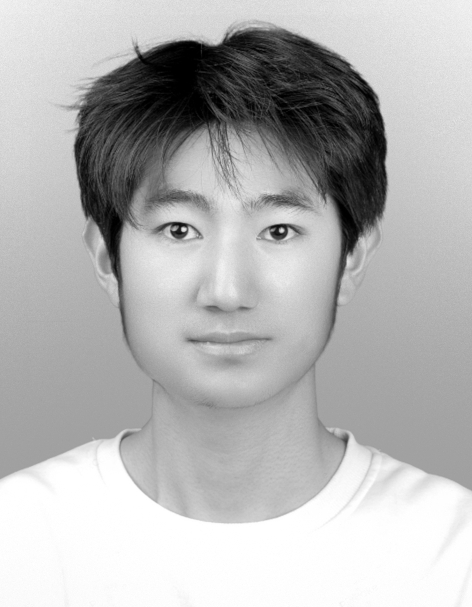
\includegraphics[height=2in,width=1in,clip,keepaspectratio]{ShuolongChen_grey.jpg}}
	 \noindent{\bfseries Shuolong Chen}\emph{
	 received the B.S. degree in geodesy and geomatics engineering from Wuhan University, Wuhan China, in 2023.
	 He is currently a master candidate at the school of Geodesy and Geomatics, Wuhan University. His area of research currently focuses on integrated navigation systems and multi-sensor fusion.
	 Contact him via e-mail: shlchen@whu.edu.cn.
	 }}
	\end{tcolorbox}
		
		
\end{document}
